\documentclass[tikz,border=7pt]{standalone}
\usepackage[T1]{fontenc}
\usepackage{lmodern}
\usetikzlibrary{arrows.meta,shapes.geometric}
\definecolor{navy}{HTML}{17334F}
\definecolor{teal}{HTML}{176E68}
\begin{document}
\sffamily
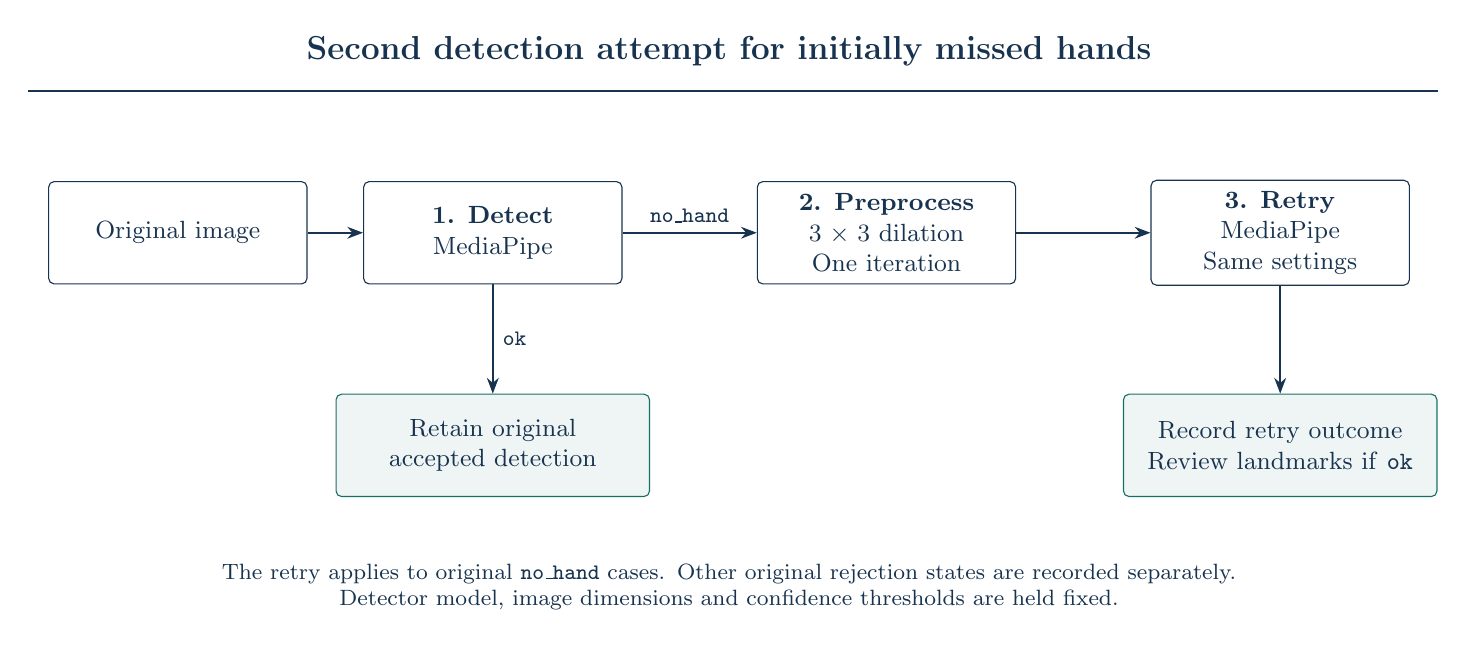
\begin{tikzpicture}[
 text=navy, font=\small,
 box/.style={draw=navy,rounded corners=2pt,align=center,minimum height=13mm,text width=30mm,inner sep=4pt},
 result/.style={box,fill=teal!7,draw=teal,text width=37mm},
 flow/.style={-{Stealth[length=2mm]},draw=navy,line width=.7pt}
]
\node[font=\large\bfseries] at (7,2.3) {Second detection attempt for initially missed hands};
\draw[navy] (-1.9,1.8)--(16,1.8);
\node[box] (input) at (0,0) {Original image};
\node[box] (detect) at (4,0) {\textbf{1. Detect}\\MediaPipe};
\node[box] (filter) at (9,0) {\textbf{2. Preprocess}\\\(3\times3\) dilation\\One iteration};
\node[box] (retry) at (14,0) {\textbf{3. Retry}\\MediaPipe\\Same settings};
\draw[flow] (input)--(detect);
\draw[flow] (detect)--node[above,font=\footnotesize]{\texttt{no\_hand}}(filter);
\draw[flow] (filter)--(retry);
\node[result] (retain) at (4,-2.7) {Retain original\\accepted detection};
\draw[flow] (detect)--node[right,font=\footnotesize]{\texttt{ok}}(retain);
\node[result] (review) at (14,-2.7) {Record retry outcome\\Review landmarks if \texttt{ok}};
\draw[flow] (retry)--(review);
\node[align=center,font=\footnotesize,text width=140mm] at (7,-4.5)
 {The retry applies to original \texttt{no\_hand} cases. Other original rejection states are recorded separately.\\
 Detector model, image dimensions and confidence thresholds are held fixed.};
\end{tikzpicture}
\end{document}
